\section{Enhancing JIVE}\label{enhJive}
%todo: referanser til artikler og ordliste, legg til figurer for å forklare bedre

In this section I will first explain the various features of JIVE, before identifying any shortcomings, and finally suggest improvements.

\subsection{Features}\label{jiveFeatures}

\begin{figure}[H]
	\centering
	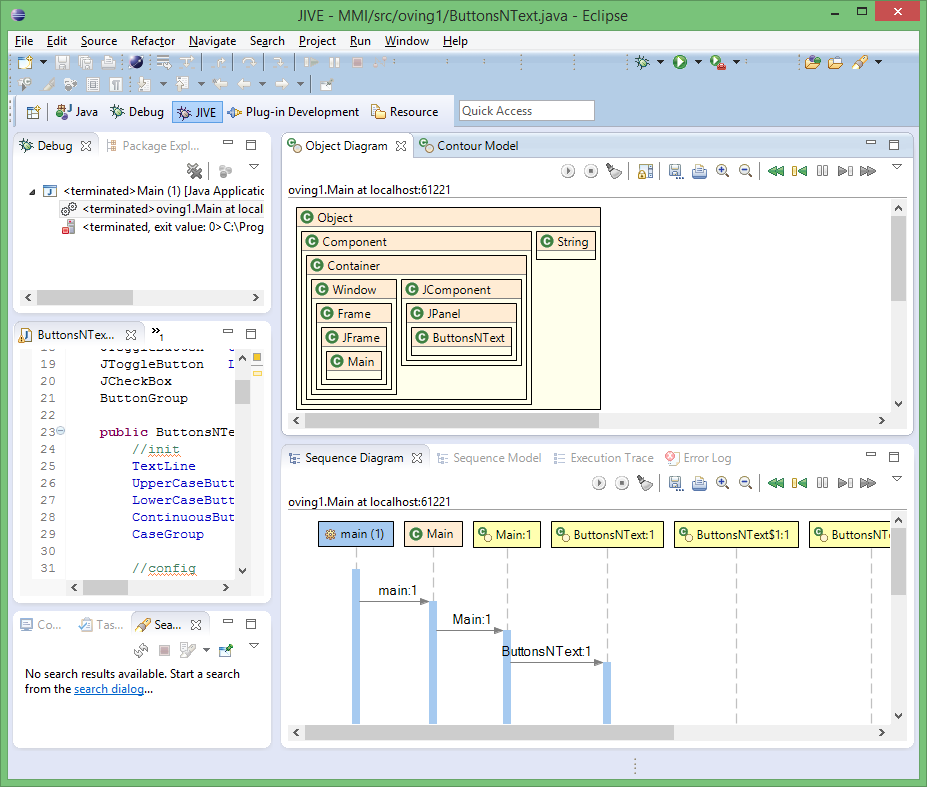
\includegraphics[width=\textwidth]{UIjivePerspective3}
	\caption{The JIVE perspective in Eclipse}
	\label{fig:UIjivePerspective}
\end{figure}
As mentioned in the prestudy, JIVE installs as a plugin in the eclipse IDE, adding another perspective in the environment shown in \autoref{fig:UIjivePerspective}.
The default views shown in this perspective are the "object diagram" and "sequence diagram" views, making the diagrams generated during debugging JIVEs two most apparent features.
The diagrams are updated according to the current state of the debugged program, so that the backtracking functionality allows you to see the entire execution graphically step-by-step.
The other views provided by JIVE are as follows: "contour model", "sequence model", "execution trace" and "search".
~\\

\begin{figure}[H]
	\centering
	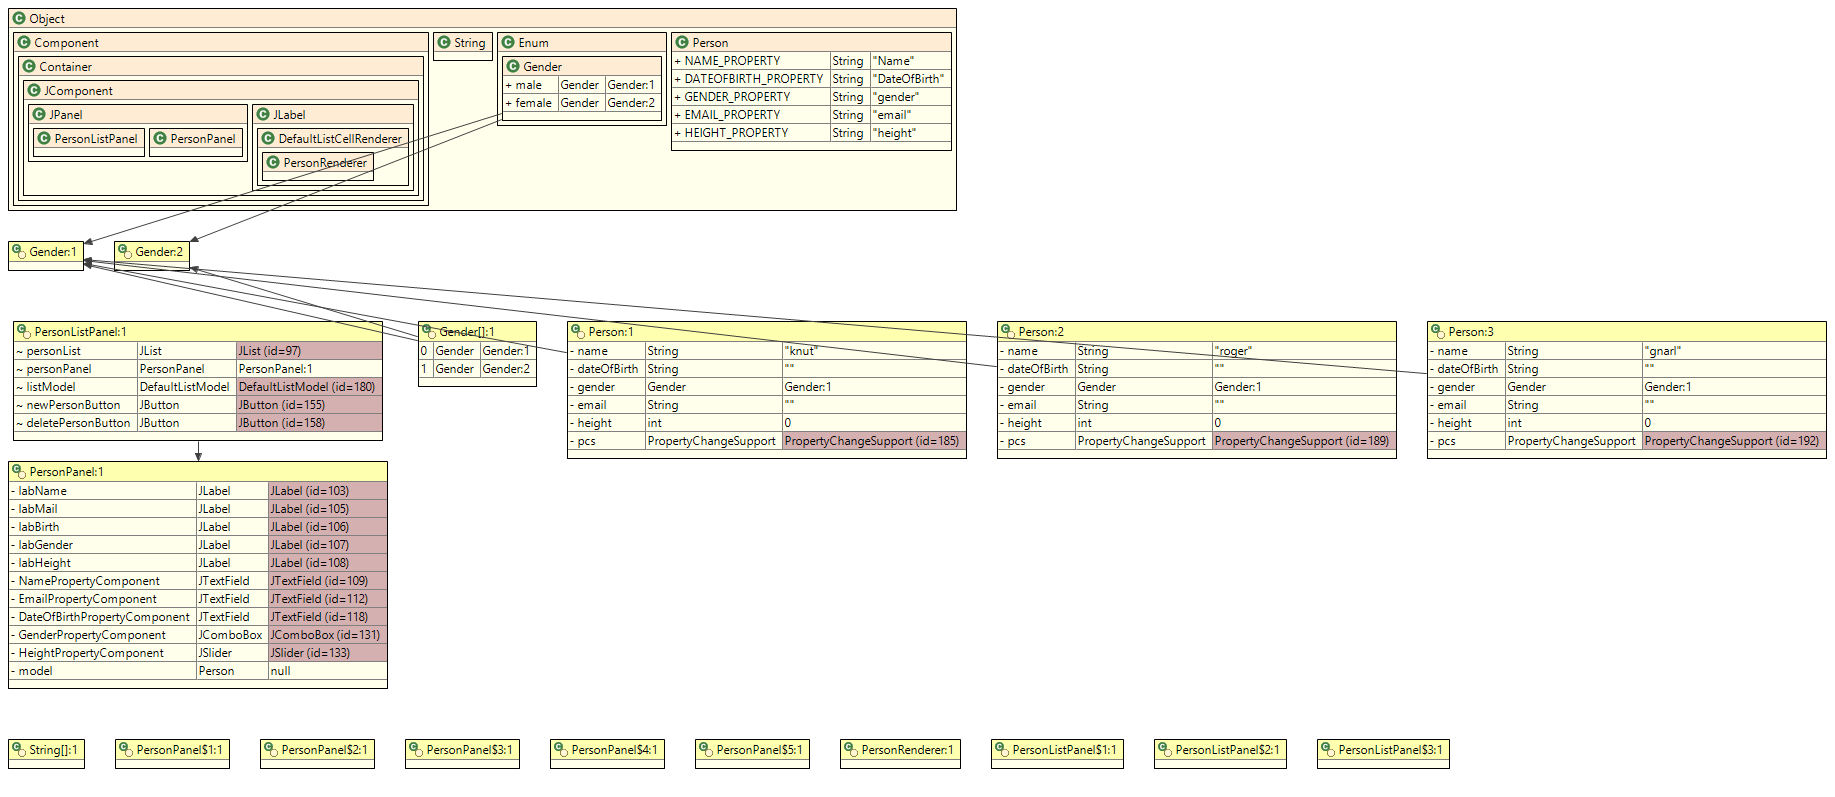
\includegraphics[width=\textwidth]{MMI-Oving4-ObjectDiagInit}
	\caption{A contour diagram generated by JIVE}
	\label{fig:conOving4Init}
\end{figure}
The object diagram-view shows the current state of the program by using a contour-diagram.
Contour-diagrams, as shown in \autoref{fig:contOving4Init}, are based on an old technique to give semantics to Algol-like languages.
The basis has been extended to support modern concepts, such as object-oriented programming.
Objects are represented by a box, or contour.
Within the contour, the objects variables are shown, with name, type and value.
The contour also uses arrows to point at other contours that are related, e.g. an other object representing the value of a variable, or an enumerator.
Inheritance is shown by putting the contour of an object within the contour of the extended object. 
Object instances are kept separate from the contours representing inheritance, but will have relational links when necessary.
Method calls are also represented in the diagram, in their own contours, linked to the calling object.
JIVE offers to hide some of the information, such as inheritance or the composition of objects, in order to make the diagram smaller, and easier to read.
Something that can be especially useful when working with larger programs, with many objects and relations.
Visibility is aided by the use of colors to highlight specific elements of the diagram, such as variables bound to objects, and method-calls.
~\\

\begin{figure}[H]
	\centering
	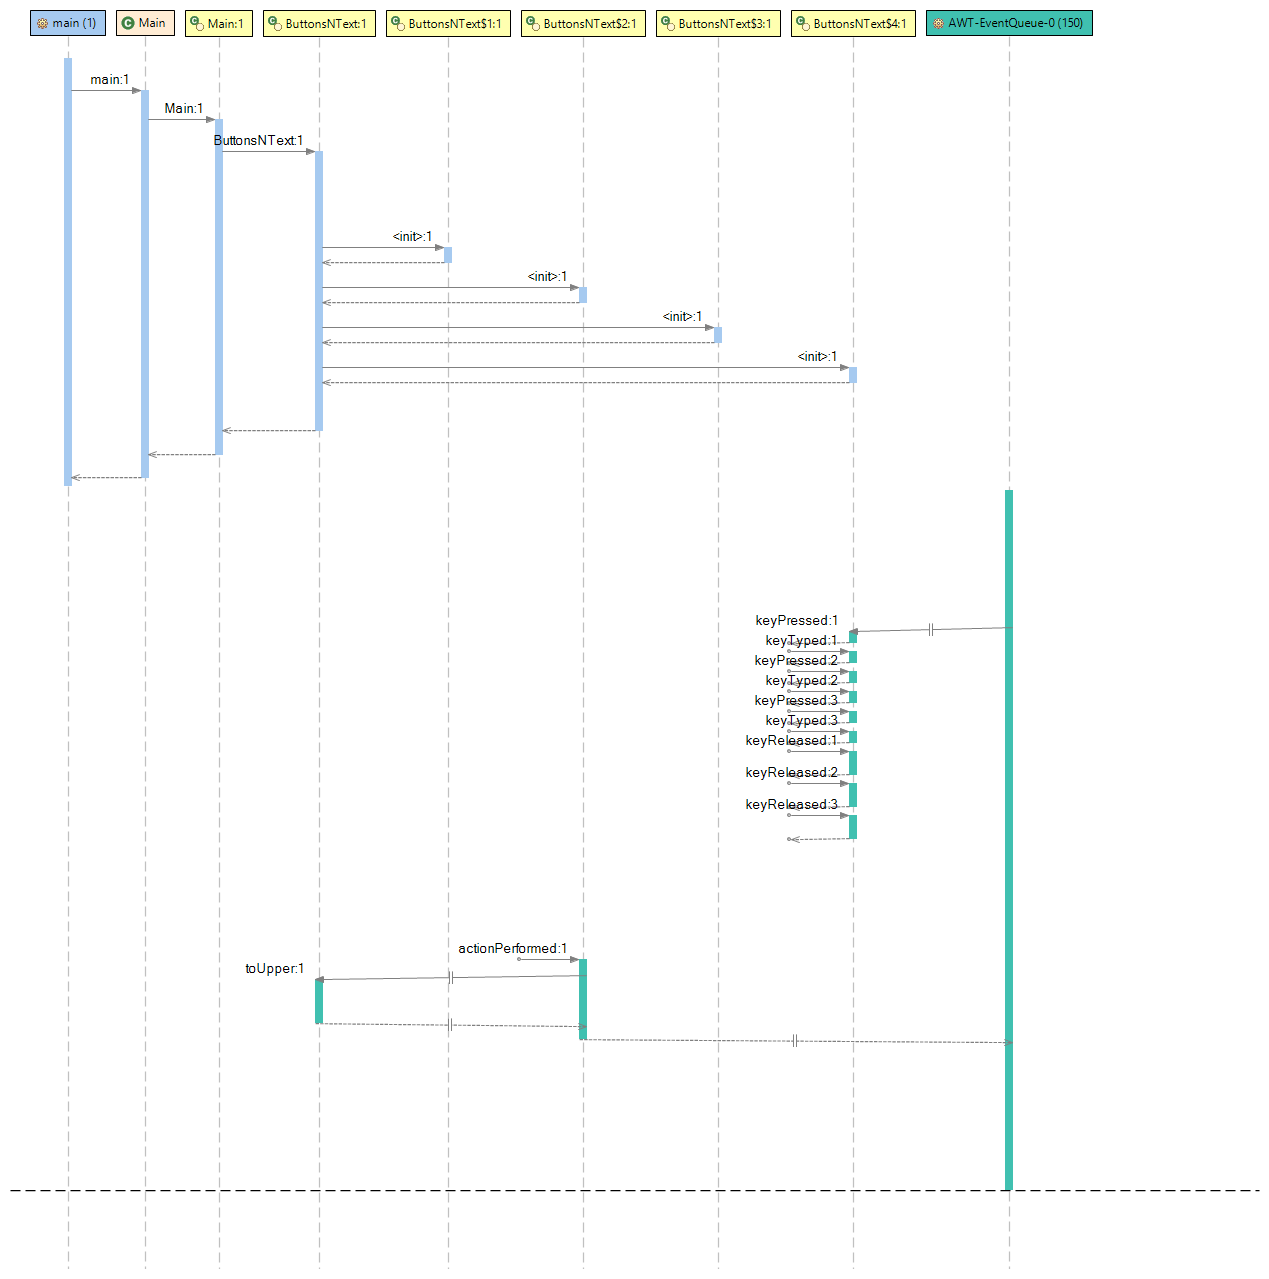
\includegraphics[width=\textwidth, trim=0 0cm 0 0, clip]{MMI-Oving1-SequenceDiag}
	\caption{A sequence diagram generated by JIVE, while running an instance of MMI-Exercise 1}
	\label{fig:seqOving1}
\end{figure}
The sequence diagrams, shown in \autoref{fig:seqOving1}, are fairly standard, with threads and objects represented by boxes on a row at the top, each with a vertical life-line.
The actual sequence is shown with a thicker lifeline, with arrows representing method-calls.
In order to differentiate the threads where the execution is happening, the sequences are colored with the same color as the thread- box the sequence originates from, regardless of witch objects and methods are involved.
In \autoref{fig:seqOving1}, one can clearly see the two colors representing the main- and the AWT-event-thread, and how elements in the diagram are colored by their parent thread.
\begin{figure}[H]
	\centering
	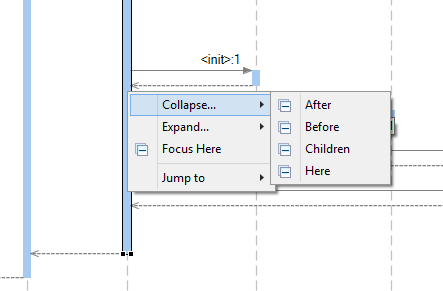
\includegraphics[scale=0.9]{UIseqRightClick}
	\caption{The sequence diagram right click menu}
	\label{fig:UIseqRightClick}
\end{figure}
Right-clicking on a lifeline offers the ability to collapse method-calls originating from that lifeline in order to hide unnecessary information, shown in \autoref{fig:UIseqRightClick}.
The collapse-menu offers four options when used on the lifeline of an object: after, before, children and here.
Before and after collapses lifelines that occurred before or after the selected event, at the same depth in the sequence-tree.
Children collapses all events that are children of the selected event, while here collapses the selected event.%figurer!
Right clicking on an object instance at the top of the diagram also offers to collapse that objects entire lifeline, the result of which can be seen in \autoref{fig:seqOving4Collapse}.
The same options are of course available for expanding collapsed elements.
Right-clicking also offers to set the execution-state via the jump-option, updating the contour-diagram and -model to show that state.
~\\

\begin{figure}[H]
	\centering
	\begin{subfigure}{\textwidth}
		\centering
		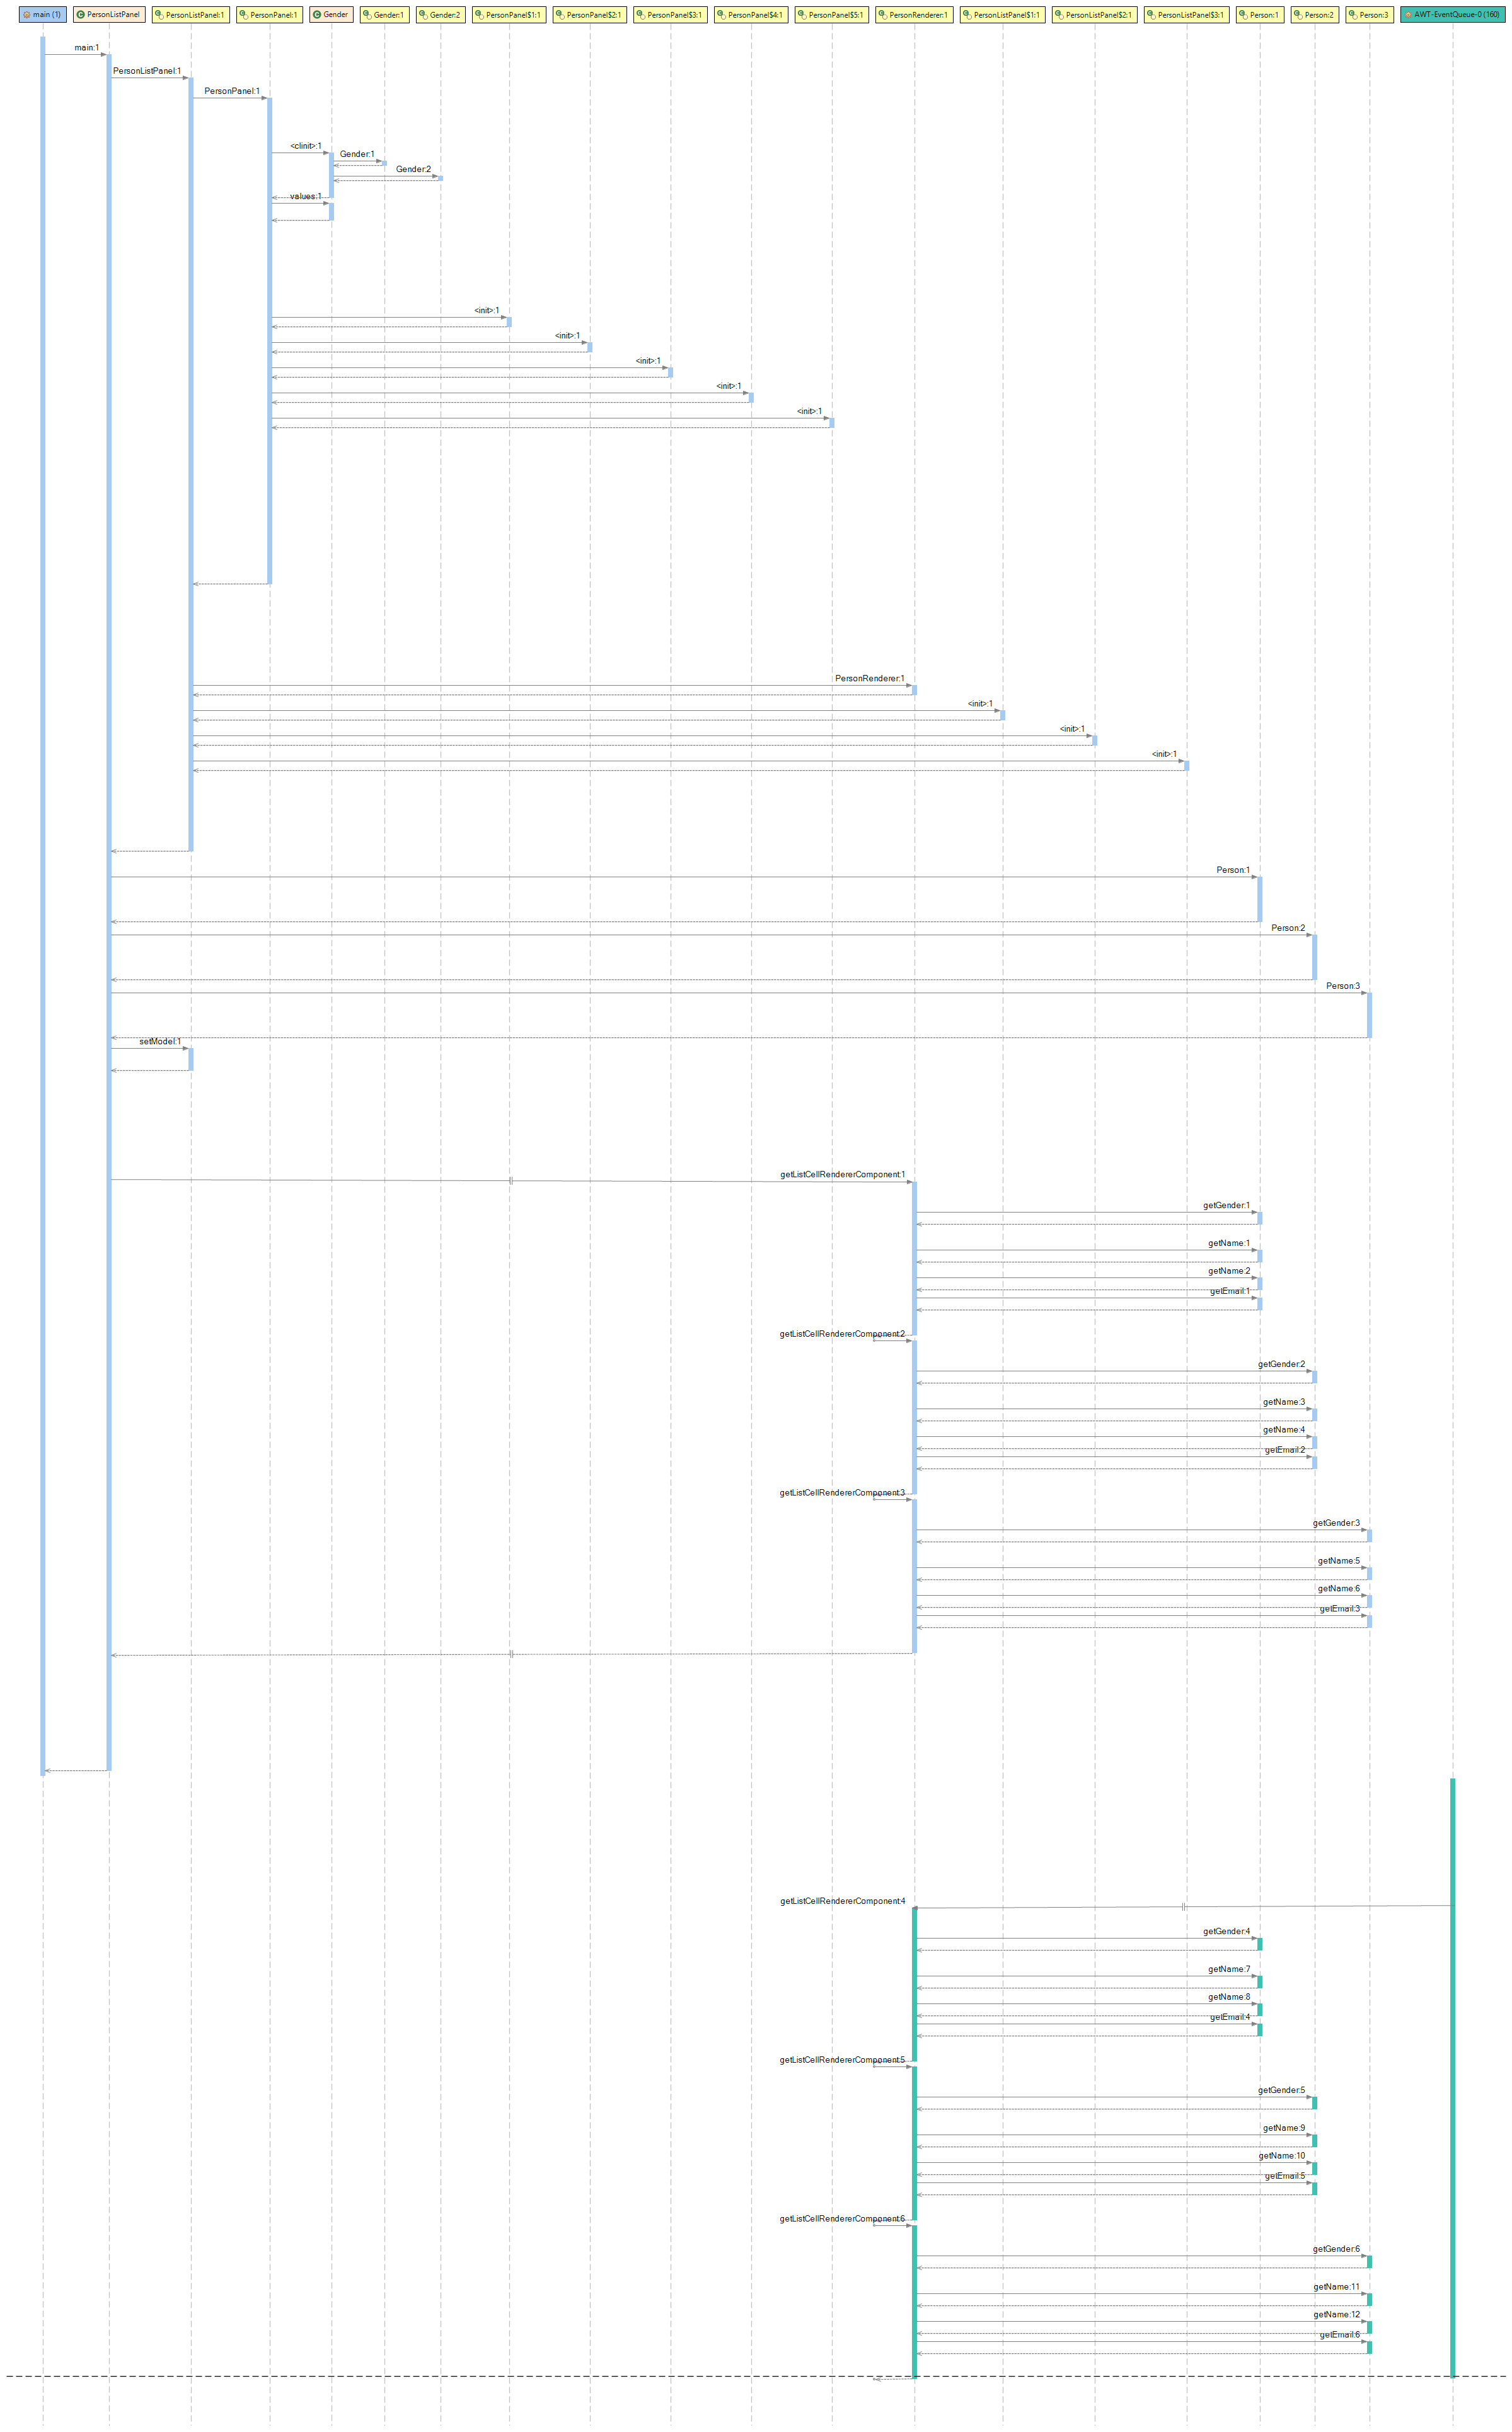
\includegraphics[width=\textwidth, trim= 0 48cm 0 50cm, clip]{MMI-Oving4-SequenceDiagInit}
		\caption{Normal}
		\label{fig:seqOving4CollapseA}
	\end{subfigure}
	\begin{subfigure}{\textwidth}
		\centering
		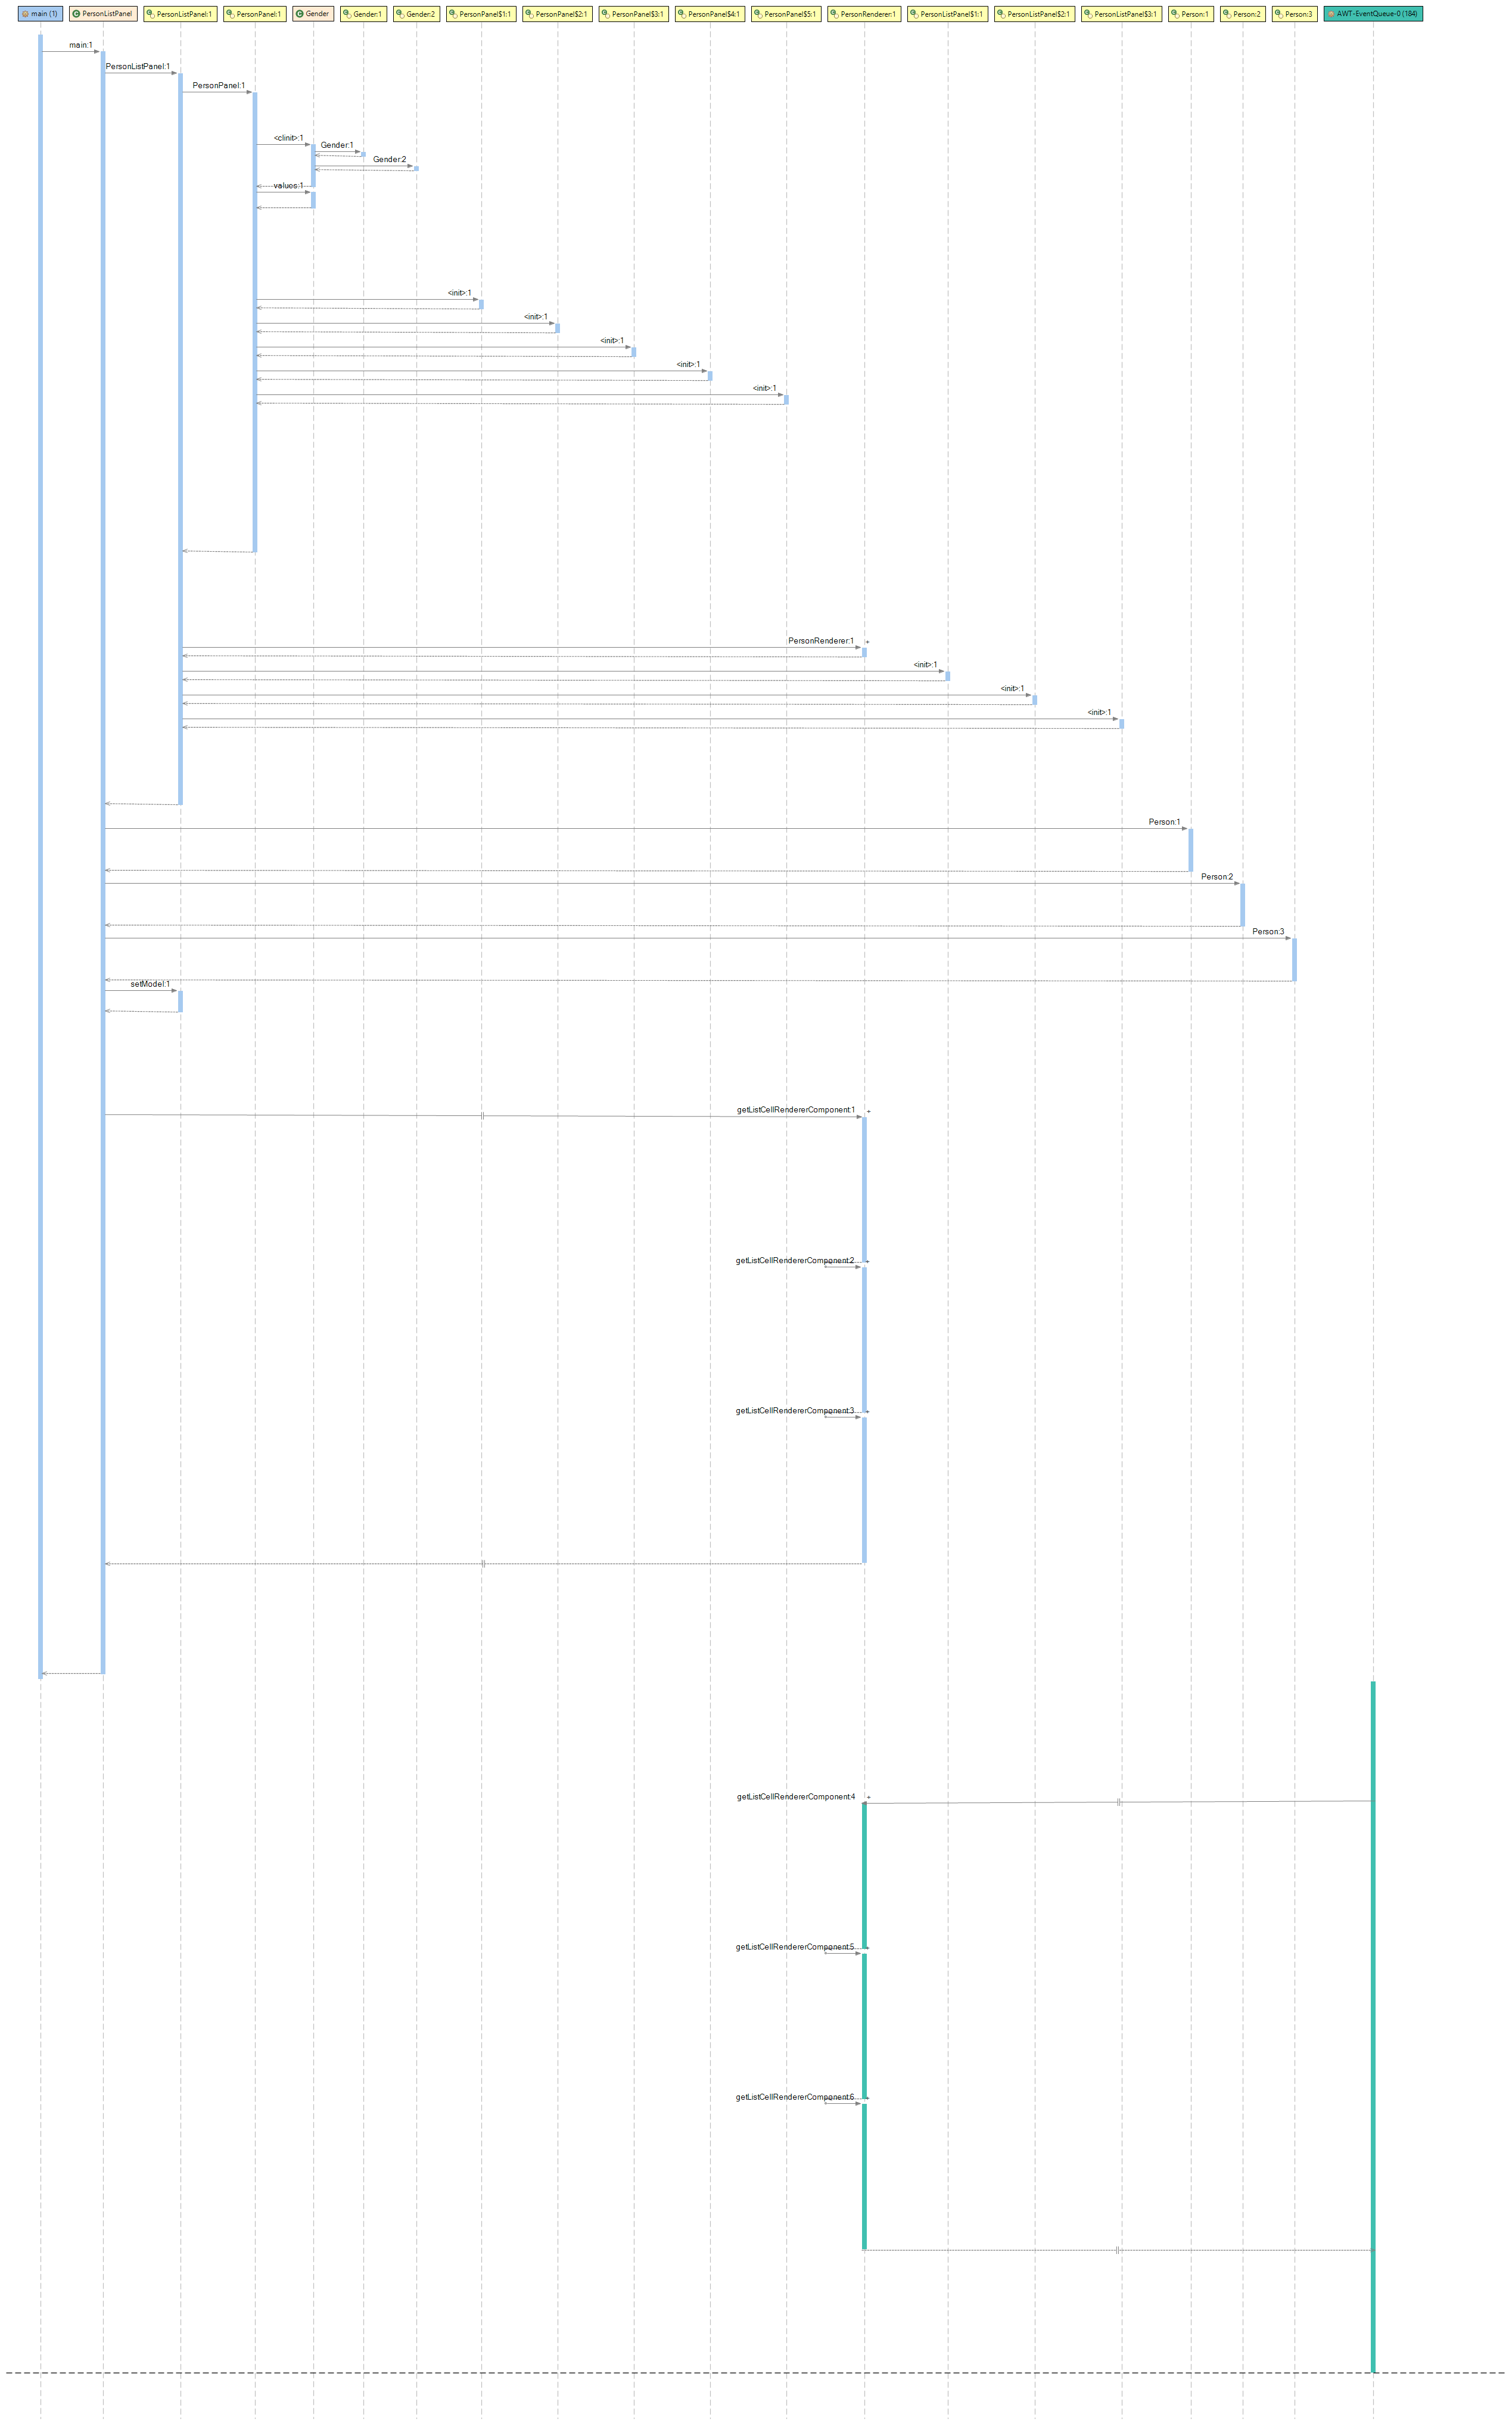
\includegraphics[width=\textwidth, trim= 0 48cm 0 50cm, clip]{MMI-Oving4-SequenceDiagInitCollapsed}
		\caption{Collapsed}
		\label{fig:seqOving4CollapseB}
	\end{subfigure}
	\caption{Normal and collapsed section of a sequence diagram}
	\label{fig:seqOving4Collapse} 
\end{figure}

Both of the diagrams can be saved as a high-resolution image at any time, so that one can look at diagrams from earlier runs, instead of being forced to view them through JIVE.
This also helps to visualize any changes made to a program, and to see what the effects are on the program flow.
They also share the ability to zoom in and out, further helping with the handling of larger diagrams.
~\\

Closely related to the diagrams, is the ability to quickly jump backwards and forwards between execution states.
This is enabled by the trace-log, containing an entry for every single event that occurs during execution of a program.
Each event is assigned an identifying number, in ascending order, and information about thread, type, caller, target, and the location of the source-code is stored.
The log is used as the basis for the models that make up the diagrams, and can be saved as both XML- and CSV-files for later use.
As mentioned in the Prestudy, logging every event has a significant impact on run-time performance, limiting the size of the programs that can be used in a meaningful way.
On the other hand, it allows the almost instant jumping between recorded states, as opposed to techniques that save a snapshot at predefined intervals, requiring the program to be run from the snapshot-state to the desired one, even if it is just a single step backwards.
~\\

The model-views each display an alternate view of their respective diagrams.%figur
They show the data-model representing the diagrams in a hierarchical structure, much like the organization of files and folders.
Right-clicking on an event in the sequence model allows you to set the execution state to that event, and have the diagrams updated accordingly.
Clicking on elements in the contour-model allows you to inspect the values of objects and their variables.
~\\

Finally, the trace-log enables the use of queries to search for specific events in the execution.
The queries are presented through a new tab in the eclipse search-window as seen in \autoref{fig:UIjiveSearchPanel}, easily accessible through the search-view, and comes with several pre-defined templates to simplify searching.
For example, searching for when a certain variable gets a certain value, only requires the user to specify the variable-name, its parent, and the value.
\begin{figure}[H]
	\centering
	\includegraphics[width=\textwidth]{UIjiveSearch}
	\caption{The JIVE search panel}
	\label{fig:UIjiveSearchPanel}
\end{figure}
~\\

\subsubsection{In Development}\label{jiveInDev}

Regex folding and state-diagrams go here.


\subsection{Shortcomings of JIVE}\label{jiveShortcomings}

Even though JIVE offers several useful features, there is still room for improvements, both for general use, and more tailored towards development of graphical interfaces, as is the focus of the MMI-course.
~\\

The diagrams are possibly the most useful feature of JIVE, showing a lot of information in an understandable way, and offering some useful interaction.
But there is still room for improvement:
Inner types are displayed with their automatically generated, and fairly anonymous, name unless given a proper name in code.
By default, most of the classes defined by the JRE itself are ignored, omitting potentially important information in GUI-applications.
For the sequence-diagrams, it is naturally not important no show the internal behavior of every object, but they are also hidden in the contour-diagram.
Related to this, is the lack of visual connections between standard-objects, and for example instances of listeners added to them.
More related to the target group for this project, is a lack of differentiation between the different object-types in typical graphical architectures.
Especially MVC, whitch is a major focus of the MMI-course, has certain distinct types that are more important than others.
~\\

The sequence-diagrams can quickly become huge and hard to navigate, and the zooming function has very few levels outward, as well as leaving all text to small to read when zooming out.
Additionally there does not seem to be any way to vertically compact the sequence-diagrams, making them unnecessarily long in cases where calls to ignored or hidden methods are being made.
For instance when horizontally collapsing large parts of the diagram, leaving the parent lifeline at the same length as before, as can be seen in \autoref{fig:seqOving4CollapseB}.
Some of the papers on JIVE mention regex-folding,that could be used to substitute a series of events with a single new event, but it is nowhere to be found in the latest version of the plugin.
~\\

Another potential for improvement is the process of stepping through recorded states, which currently requires manual interaction for each step, making complete replays of an execution infeasible due to the massive number of events recorded even for simple programs.
~\\

The search-view, while useful, is very strict in terms of what it looks for.
For example, searching for the creation of an object requires its full name, including packages, so searching for creations of JButton-instances would require a search for javax.swing.JButton.
~\\

\subsection{Suggestions for improvement}\label{jiveSuggestions}

Based on the mentioned shortcomings, the following improvements are suggested.
~\\

The ability to detect an inner type with a generic name, and display its parent type in the diagrams instead of its own.
This will make, among others, listener-heavy programs much more understandable as one can see what kind of listener each object is, instead of guessing, based on when it is invoked in the sequence-diagram.
Further helping the same situation, is to visually link listeners to the objects they are added to, in the contour-diagram, making it clearly visible which object is being listened to by the different listeners.
A crude visualization of these two changes, compared to the original, can be seen in \autoref{fig:contOving4Changes}.
~\\

Finding ways to highlight the different parts of e.g. an MVC-architecture, making it clearly visible which objects make out the models, views and controllers, may further help the understanding of a program.
But such highlighting must be balanced in order to not create a visual chaos of different colors.
Adding symbols instead of colors might be a better solution, both maintaining the current color-scheme, and adding new information.
The coloring, highlighting and naming of inner types should apply to both of the diagrams.
~\\

\begin{figure}[H]
	\centering
	\begin{subfigure}{\textwidth}
		\centering
		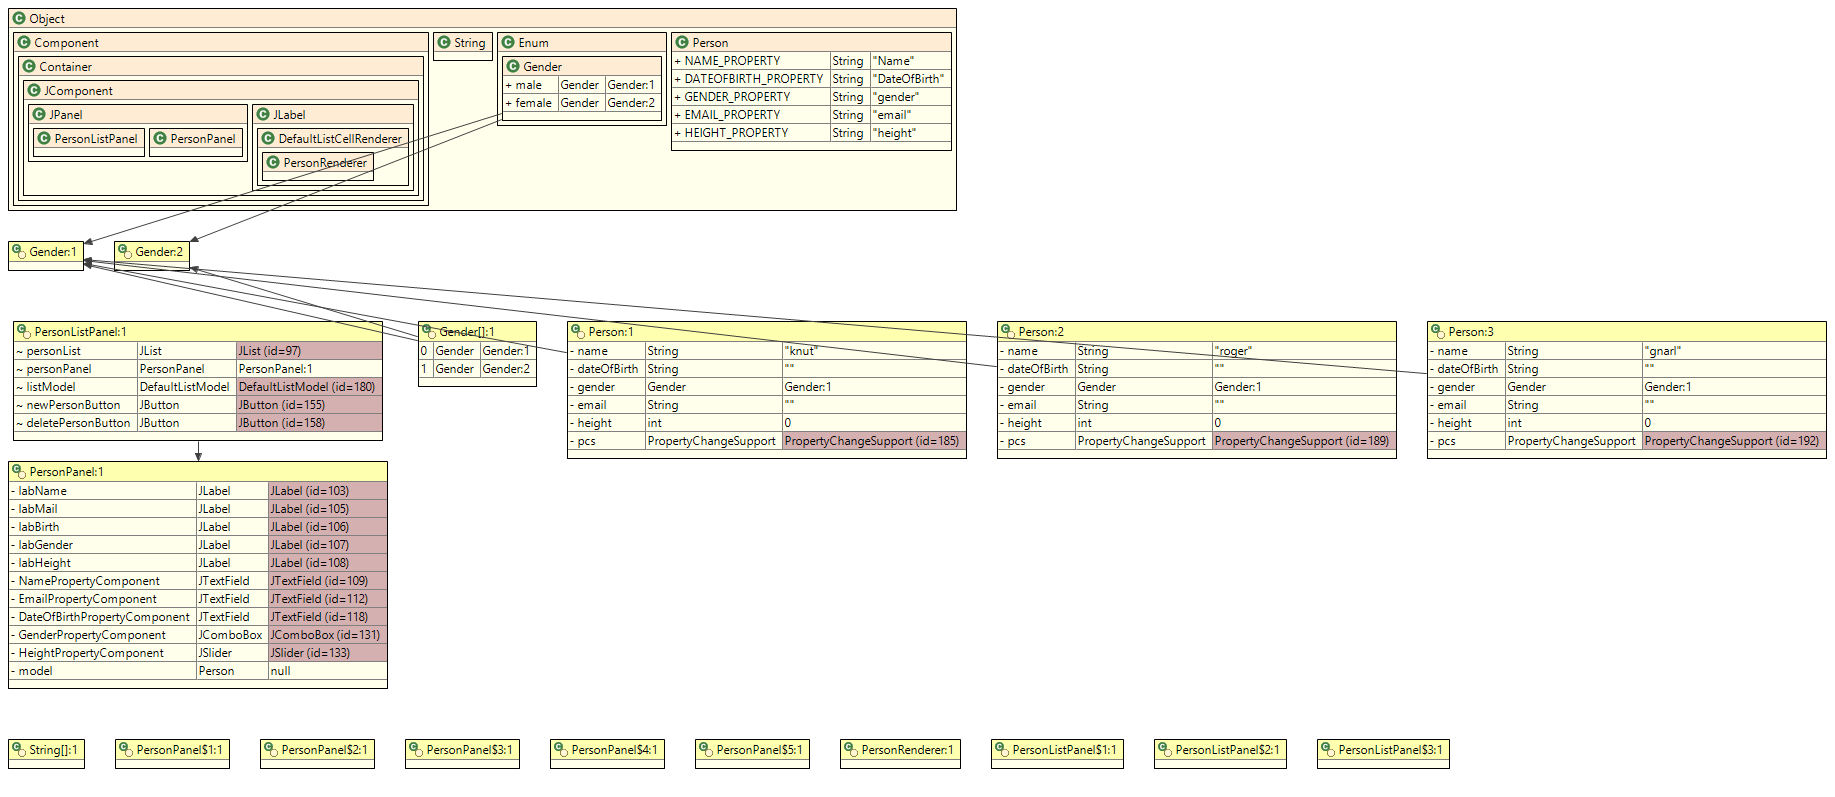
\includegraphics[width=\textwidth, trim= 0 0 0 0, clip]{MMI-Oving4-ObjectDiagInit}
		\caption{Original}
		\label{fig:contOving4ChangesA}
	\end{subfigure}
	\begin{subfigure}{\textwidth}
		\centering
		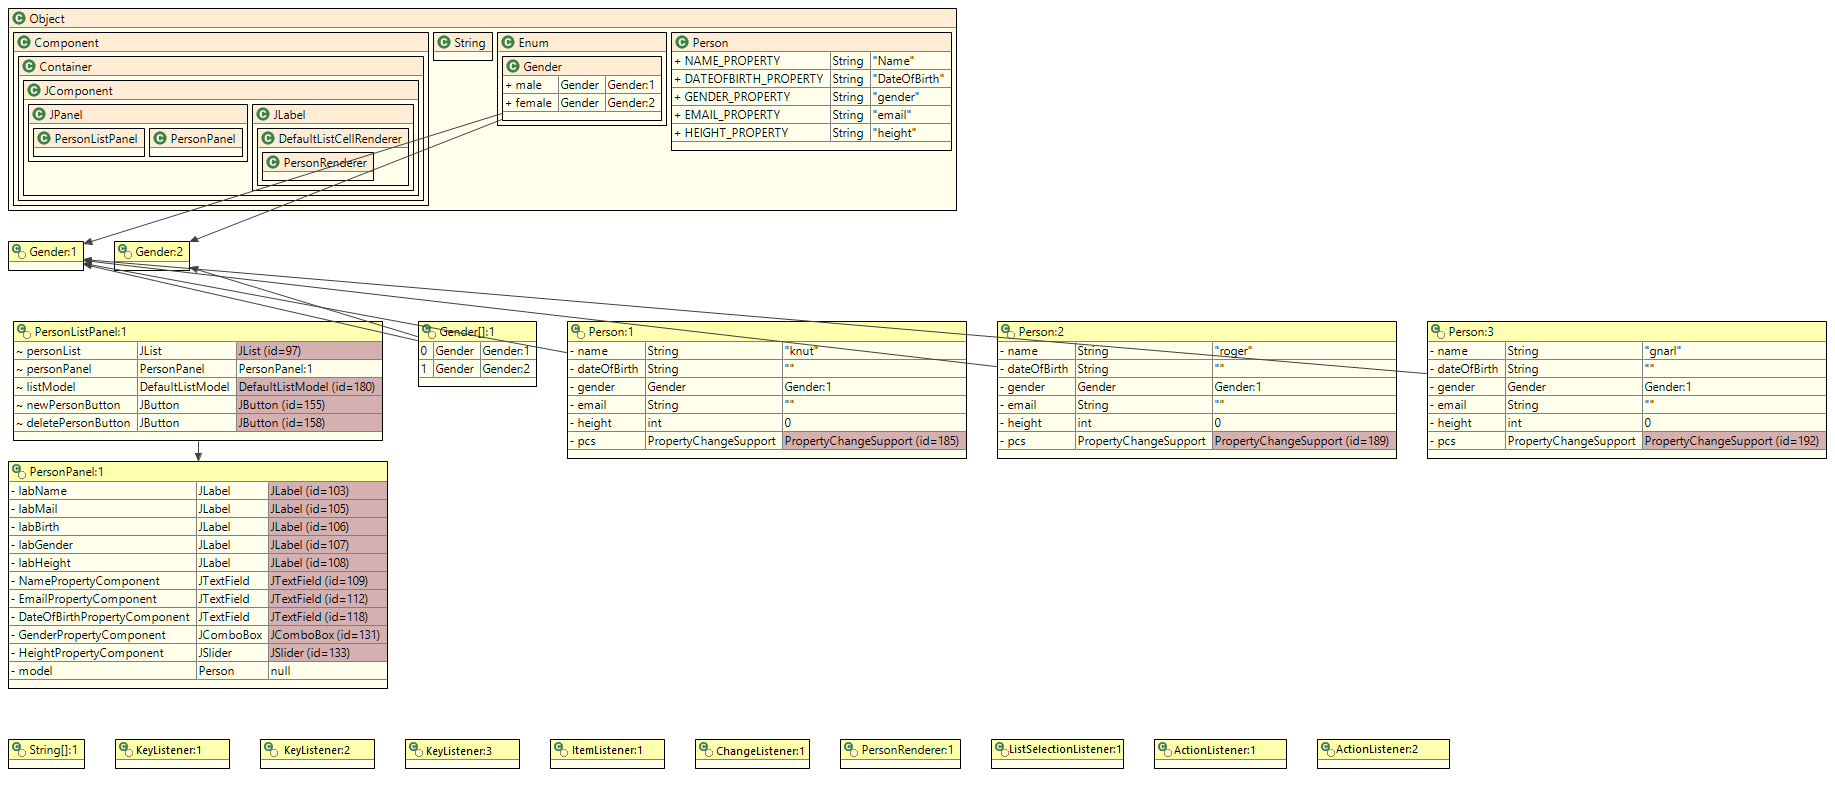
\includegraphics[width=\textwidth, trim= 0 0 0 0, clip]{MMI-Oving4-ObjectDiagInit-edit}
		\caption{Changed naming of inner types}
		\label{fig:contOving4ChangesB}
	\end{subfigure}
	\begin{subfigure}{\textwidth}
		\centering
		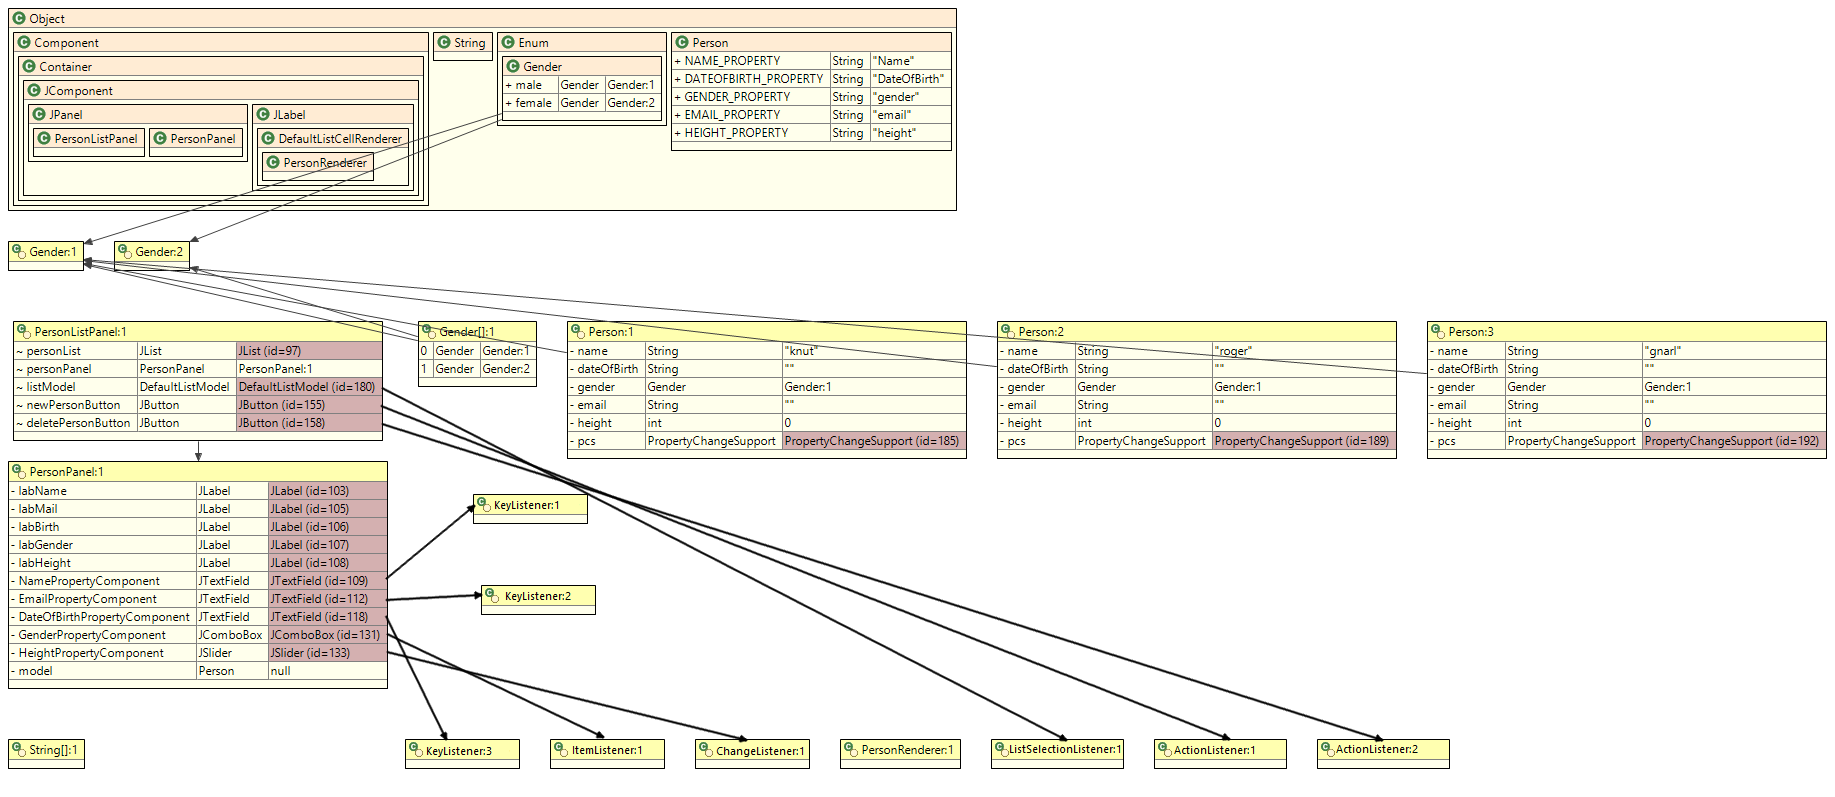
\includegraphics[width=\textwidth, trim= 0 0 0 0, clip]{MMI-Oving4-ObjectDiagInit-edit3}
		\caption{Listeners connected to the object listened to}
		\label{fig:contOving4ChangesC}
	\end{subfigure}
	\caption{Crude comparison of suggested changes to the contour diagram}
	\label{fig:contOving4Changes} 
\end{figure}

Exploring changes to the default exclusion-filter, in order to provide more useful information out of the box, is also an option.
This will provide a better experience for certain scenarios, but may be useless in other cases by providing too much unnecessary information.
A way to easily switch filters by defining presets might be preferable.
The filter might also be extended to support both exclusion and inclusion, allowing a more fine-grained selection of interesting classes.
As an example, one might be interested in ignoring the entire javax-package, but still allowing javax.swing in order to see more GUI-related objects.
It is also important to not allow too many packages through the filter, as the performance can suffer immensely from logging too many events.
~\\

Allowing more ways to interact with the diagrams, e.g. hiding elements or compressing sequences, should improve usability for larger programs and longer runs.
The way the sequence diagrams currently work, object instances are added as they appear, resulting in later method calls to draw lines crossing large parts of the diagram, as shown in \autoref{fig:seqOving4CrossLines}.
\begin{figure}[H]
	\centering
	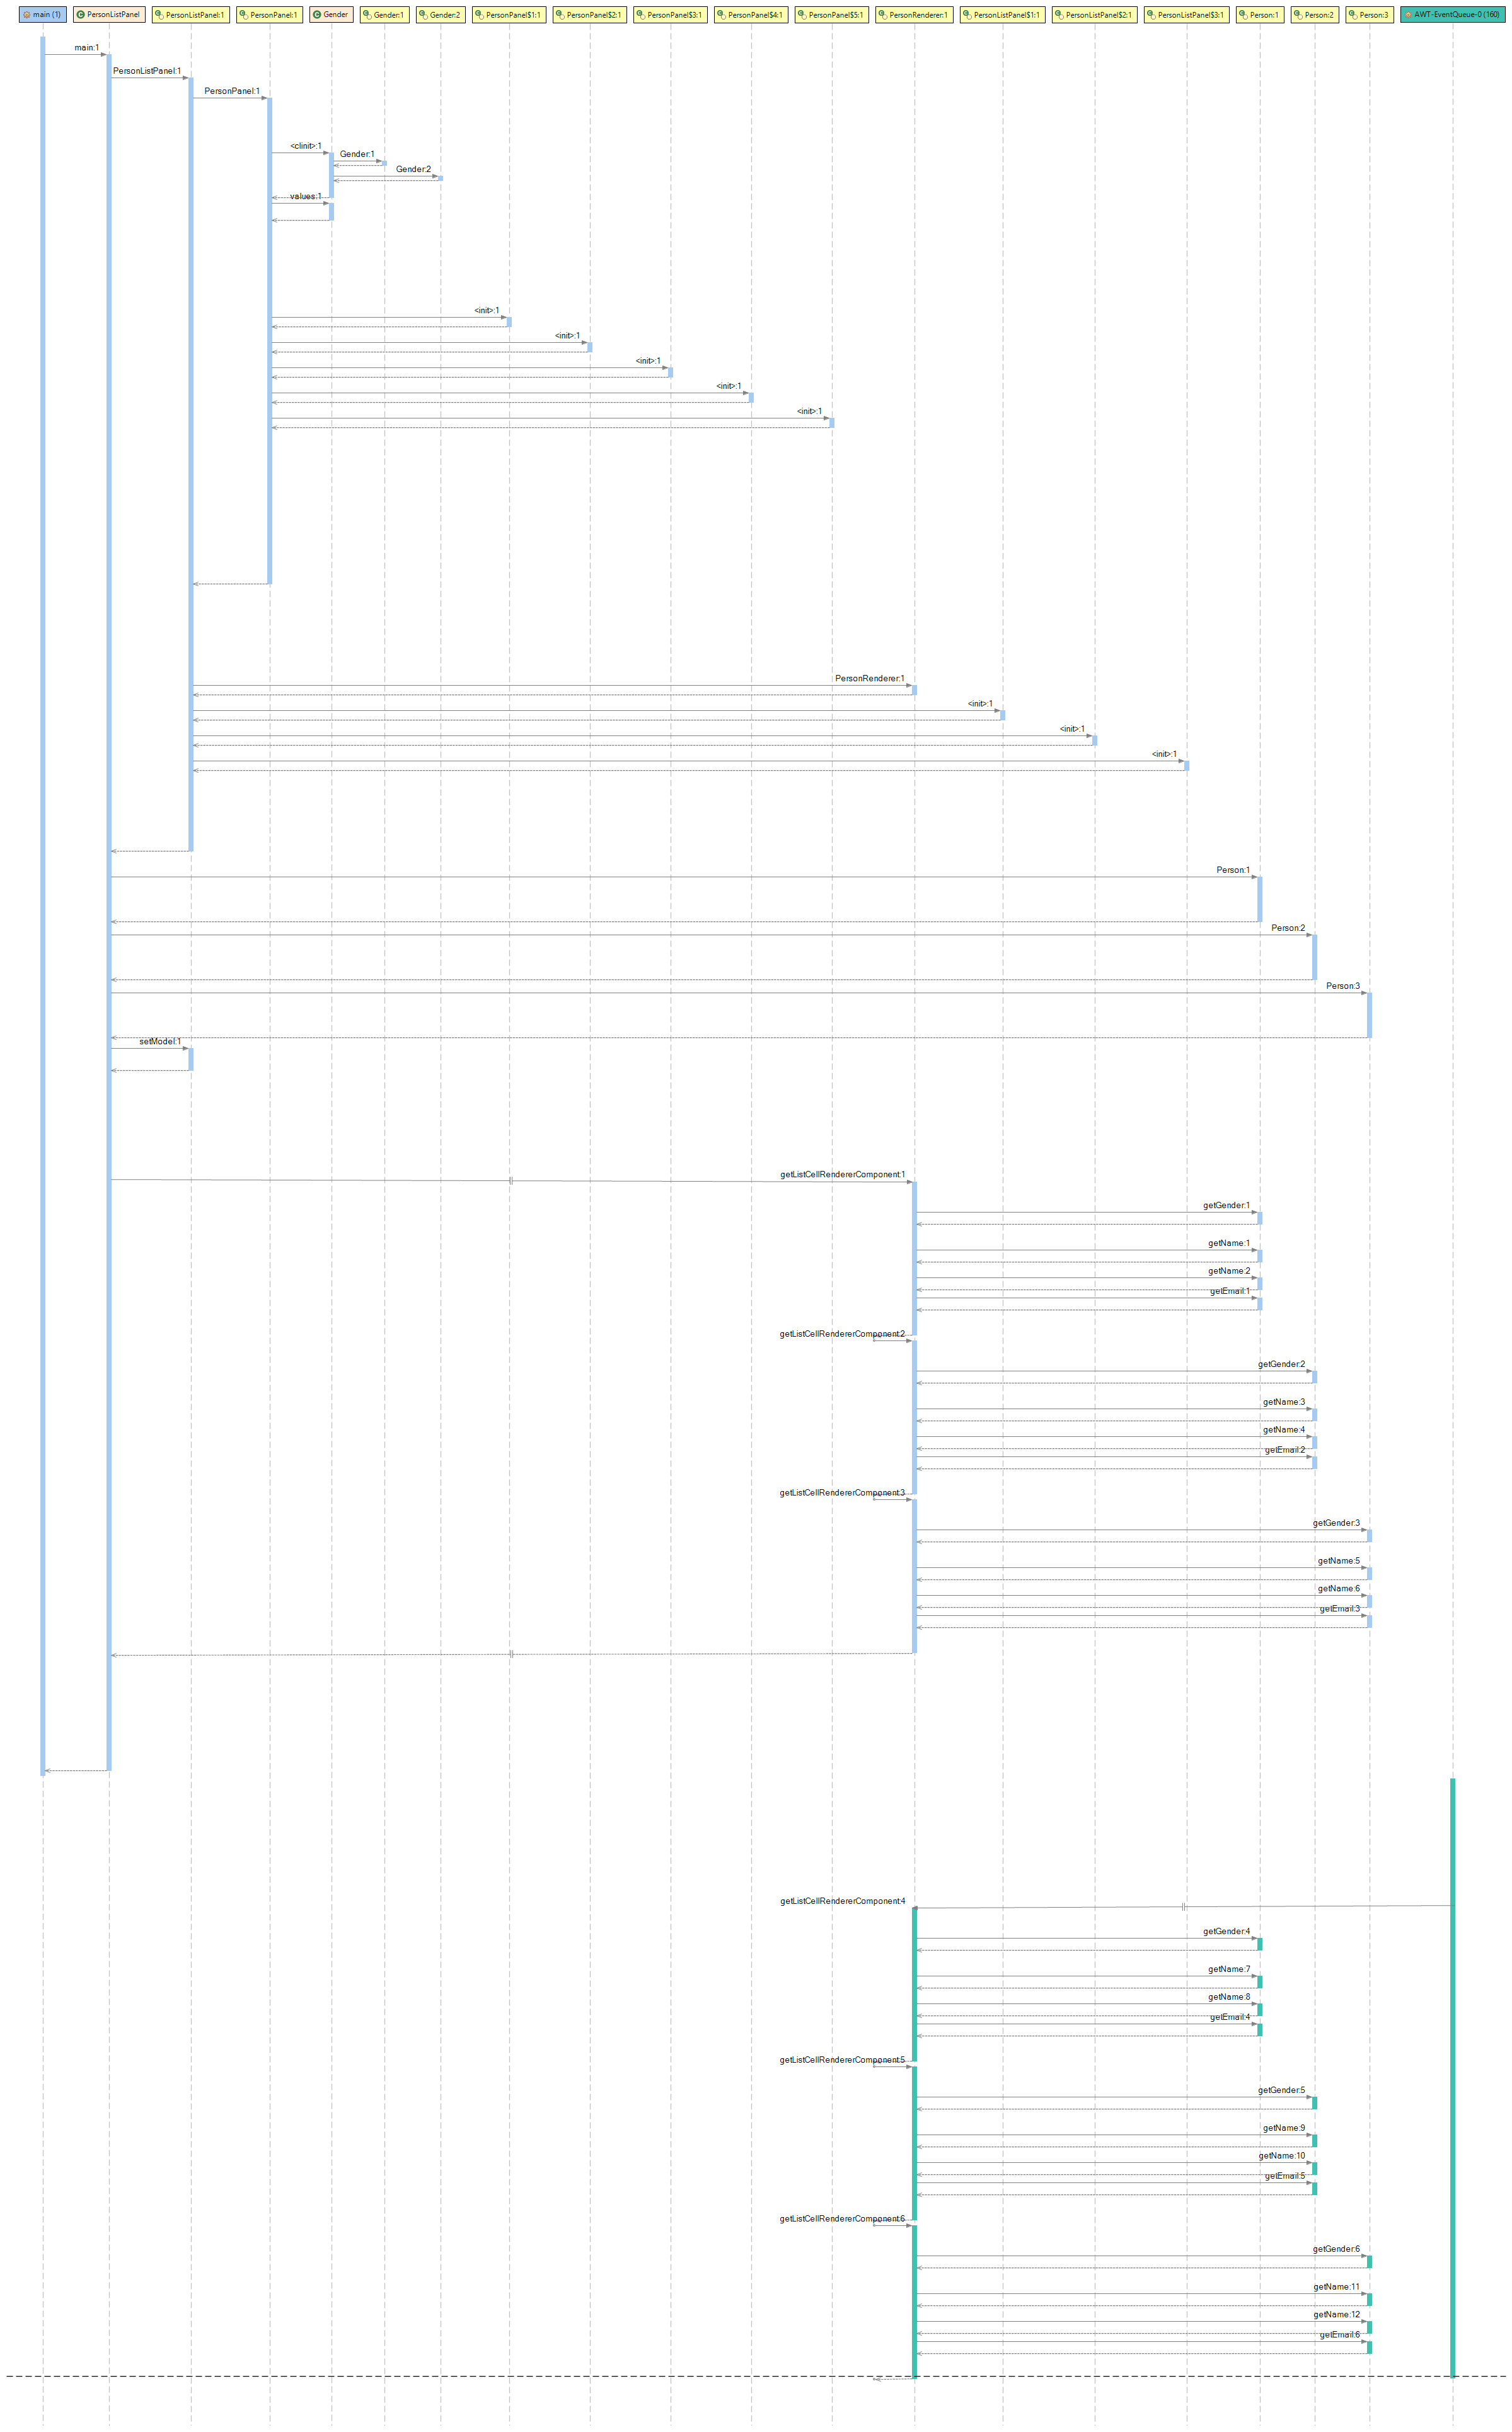
\includegraphics[width=\textwidth, trim= 45cm 0 0 100cm, clip]{MMI-Oving4-SequenceDiagInit}
	\caption{A section of a larger sequence diagram, showing method calls crossing several unrelated lifelines}
	\label{fig:seqOving4CrossLines}
\end{figure}
In the case of exploring events triggered by a listener, the ability to isolate the involved objects, and reorder the diagram could be very useful, providing a clean view of a smaller series of events.%figur?
Using the same figure as an example, the rightmost, and longest, bar would be moved to the far left, the three second-longest would be in the middle, while the shortest ones would be to the left.
In total, only the lifelines of those five objects would be visible, all the ones that are being crossed in \autoref{fig:seqOving4CrossLines} are unnecessary, and would be hidden as shown in \autoref{fig:seqOving4IsolatedMock}.
This function should be accessed by right clicking on the topmost event that is desired, and selecting a "view isolated" option.
Whether the isolated view should appear in a new eclipse view, or simply modify the existing view of the sequence diagram, is something that should be determined by user-testing.
\begin{figure}[H]
	\centering
	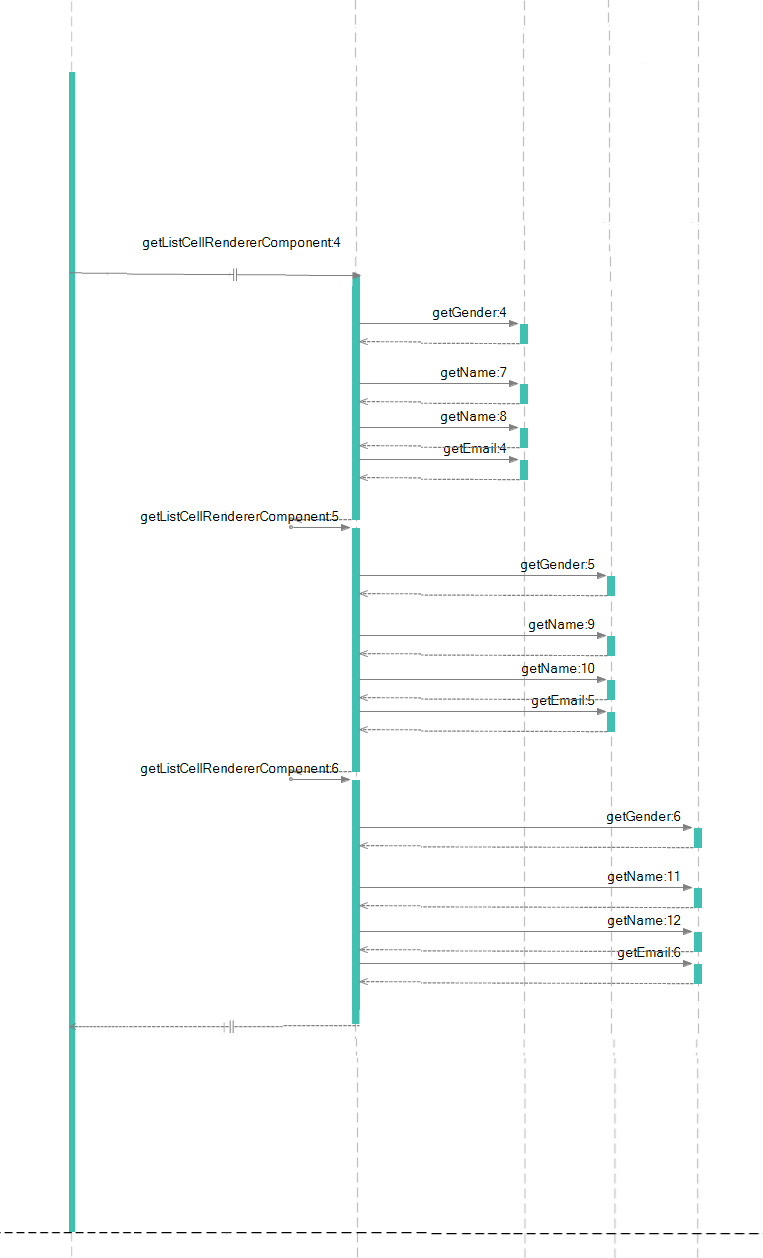
\includegraphics[height =.5\paperheight]{MMI-Oving4-SequenceDiagInit-isolatedEventsMock}
	\caption{An example of how \autoref{fig:seqOving4CrossLines} might look in the isolated view}
	\label{fig:seqOving4IsolatedMock}
\end{figure}
~\\

Stepping through the recorded states is, as mentioned above, cumbersome.
While there are quick and easy ways to jump straight to any interesting state, it may also be interesting to view a playback of a part of, or the entire execution.
This would allow an easier way of observing changes happening in a program.
The playback would automatically step through the recorded states at a pace that the user should be able to adjust, updating the diagrams for each step.
Playback should be possible to initialize from any selected event that has been recorded, as starting from the beginning would often be a waste of time.
~\\

Searching can be improved by relaxing the requirements for for search-terms.
The requirement of full class names in searches caused some confusion, and made me wonder if the feature was working at all.
Relaxing this requirement to allowing partial class names, or substrings in general, would be an improvement to the usability of the tool.
